\subsubsection{Embedding System and Router}
\label{sec:emb_sys_and_router}
The main result of this study was the creation of two key components: a flexible embedding
subsystem and a trainable router for the MoTE unit. These developments not only provide
a solid foundation for the further development of FinABYSS, but also open up a wide scope
for use in related application projects.

As part of the study, we conducted a series of experiments to select optimal combinations
of embedding models, dimension reduction methods, and clustering algorithms, using different
metrics to adjust hyperparameters. At the first stage, the basic chain consisted of ModernBERT,
UMAP (cosine metric), HDBSCAN (Euclidean metric) was optimized by the silhouette coefficient.
Despite the satisfactory results, we noted a strong dependence on the cluster structure and
the sensitivity of the silhouette to the shape of the clusters, which appeared to be arbitrary
shapes in our data.

The second stage repeated the same bundle, but the DBCV index was chosen as the target metric. Due
to the DBCV property of taking into account density features and heterogeneity of the point
distribution, hyperparameters selected for DBCV provided more semantically consistent and dense
clusters.

Finally, we tested the finely tuned STS version of ModernBERT ("gte-modernbert-base")
\parencite{MGTE2024} in combination with UMAP, but with $L_2$-Euclidean
metric, and the same HDBSCAN, also configured for $L_2$-Euclidean distance. However, this
combination was inferior to the previous one: the DBCV index was only 0.405 against 0.476
for the cosine + euclidean pair.

Additional analysis of the noise points and cluster structure confirmed this advantage. When using
the $L_2$-Euclidean metric, the proportion of noise points reached 42.16\%, and the number
of clusters was 97 (with a maximum size of 3,220 points and a minimum size of 260).
For the cosine + euclidean pair, the noise was only 36.18\%, and the number of clusters increased
to 162; at the same time, the maximum cluster increased to 3,742 points, and the minimum decreased
to 109. Thus, the "cosine + euclidean" approach demonstrated a better ratio of cluster density
and separability.

The experimental results clearly indicate the superiority of the ModernBERT + UMAP scheme with cosine
metric and HDBSCAN with Euclidean distance in the tasks of topical clustering of financial texts.
Combined with DBCV index optimization, this approach forms the most semantically coherent groups,
minimizes the proportion of noise instances, and provides a more stable basis for subsequent training
of the MoTE router.

Nevertheless, unfortunately, obvious problematic areas of the current implementation have also been
identified. The resulting clusters and their structure cannot be incrementally updated with streaming
new publications, which happens for several reasons. Firstly, the trained model is a GPU implementation
from the cuML library, in which critical errors were discovered in the code version 25.02
\parencite{cuml2020machine} only after conducting research. Secondly, the chosen UMAP algorithm
does not work well enough in incremental mode by its nature, which is why there are other implementations,
such as AlignedUMAP \parencite{mcinnes2018umap-software} or ParametricUMAP based on a neural network
as a basic model \parencite{ParametricUMAP2020}. Unfortunately, both of these implementations are available
exclusively for training on a central rather than a GPU. And there are not enough computing resources
for learning on a central processor in the context of the current study.

Thus, the bottleneck of this study and the proposed solution is the lack of computing power for training
models, which will be improved in further research.

\subsubsection{Semantic Map}
% \ref{sec:emb_sys_and_router}

Finally, based on the developed embedding subsystem and the MoTE router, a separate UMAP model was trained,
designed to translate vectors from the intermediate latent clustering space into a two-dimensional
representation convenient for visual analysis. It is this projection that underlies the Semantic Map
of Financial Publications, one of the key components of the FinABYSS interface, which provides a deep
and intuitive study of the thematic structure of news streams.

\begin{figure}[H]
    \centering
    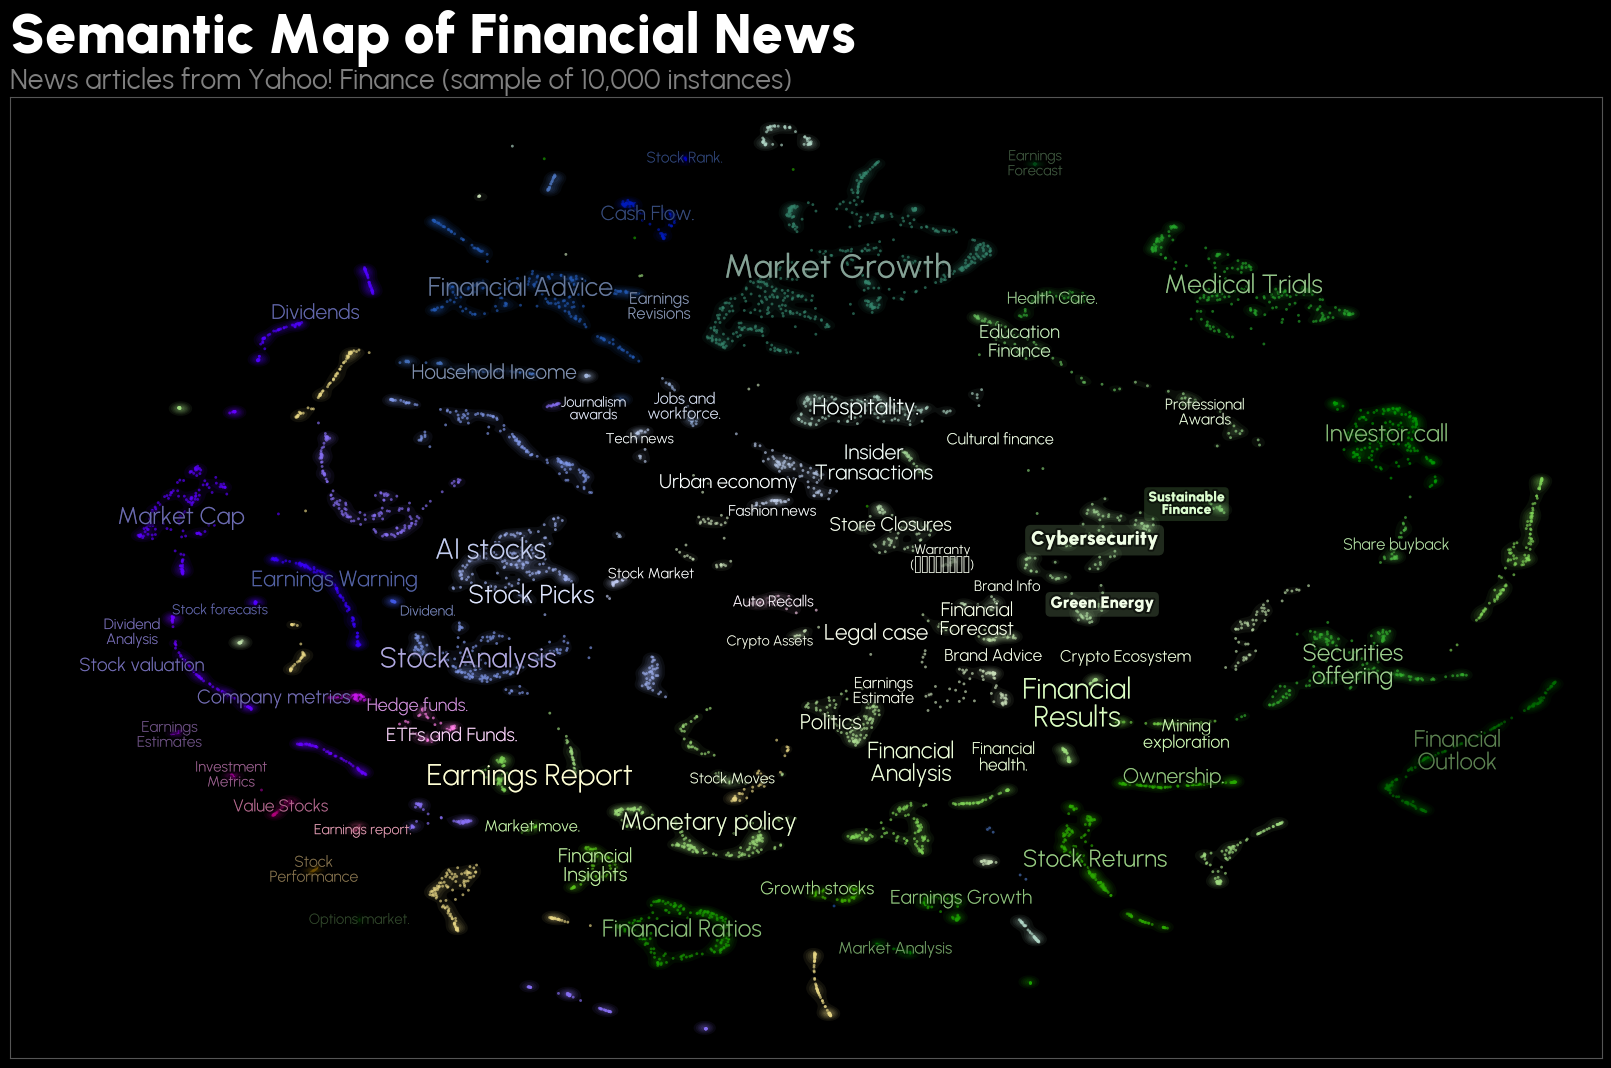
\includegraphics[width=1\linewidth]{img/semantic_map.png}
    \caption{Semantic map (early demo version) of a sample of 10,000 financial publications
    from September 17, 2023 to March 1, 2025, clustered by financial topics.}
    \label{fig:semantic_map}
\end{figure}

First, a static version of the map was implemented, which displays 100,000 financial items from September 2023
to March 2025, divided into clusters by subject (Figure \ref{fig:semantic_map}). Each cluster is marked
with an automatically generated tag word without any manual annotation. Despite the automatic nature
of the assignment, the labels turned out to be representative: dense groups of articles on healthcare,
"Sustainable Finance," "Cybersecurity," and "Green Energy" are located side by side, reflecting their semantic
proximity. The same thing happens with the "Politics" and "Monetary Policy" clusters.

However, the static map only demonstrates the potential of UMAP projection. The FinABYSS interactive Semantic
map goes far beyond the simple visualization of points:

\begin{itemize}
    \item Hovering over any point reveals the metadata of the article: title, date and time of publication,
    hierarchical topic (macro/meso/microtheme), author and source. At the same time, a preview of the full
    text and a direct link to the original publication are available.
    \item The keyword search engine allows you to quickly filter articles containing special terms. The search
    can be combined with filters by date range, publication volume, and other numerical attributes (for example,
    text volume or number of views), which makes it easier to spot historical events and triggers on the graph.
    \item The Sources and Topics section makes it possible to include and exclude news sources or target clusters,
    helping to focus on relevant publications in complex analytical scenarios.
    \item A word cloud function is also available for articles, which is formed based on the most frequent words
    found in a selected group of texts. The word cloud instantly displays the dominant terms and discussion patterns,
    which complements the quantitative outline of the graph with qualitative characteristics.
\end{itemize}

Thus, the FinABYSS semantic map is a full-fledged analytical system that combines the power of the selected UMAP
and HDBSCAN models, and with further development, the hybrid CNN-LSTM architecture and the MoE approach to sentiment
analysis. It provides the researcher with the opportunity not only to visually distinguish named clusters and
their mutual arrangement, but also to delve deeply into the content of each publication, combining automatic and
manual analysis methods.

The developed interactive Semantic map is a natural continuation of the previous FinABYSS modules. All the pipeline
links are connected in a single chain. The tool offers the user a transparent, scalable and flexibly customizable
interface for semantic research of financial news, where each element --- from cluster labels to a cloud
of words --- reflects the results of the computational logic of the system and supports expert solutions
in the analysis of market processes.

\subsubsection{Practical Importance}

\begin{figure}[H]
    \centering
    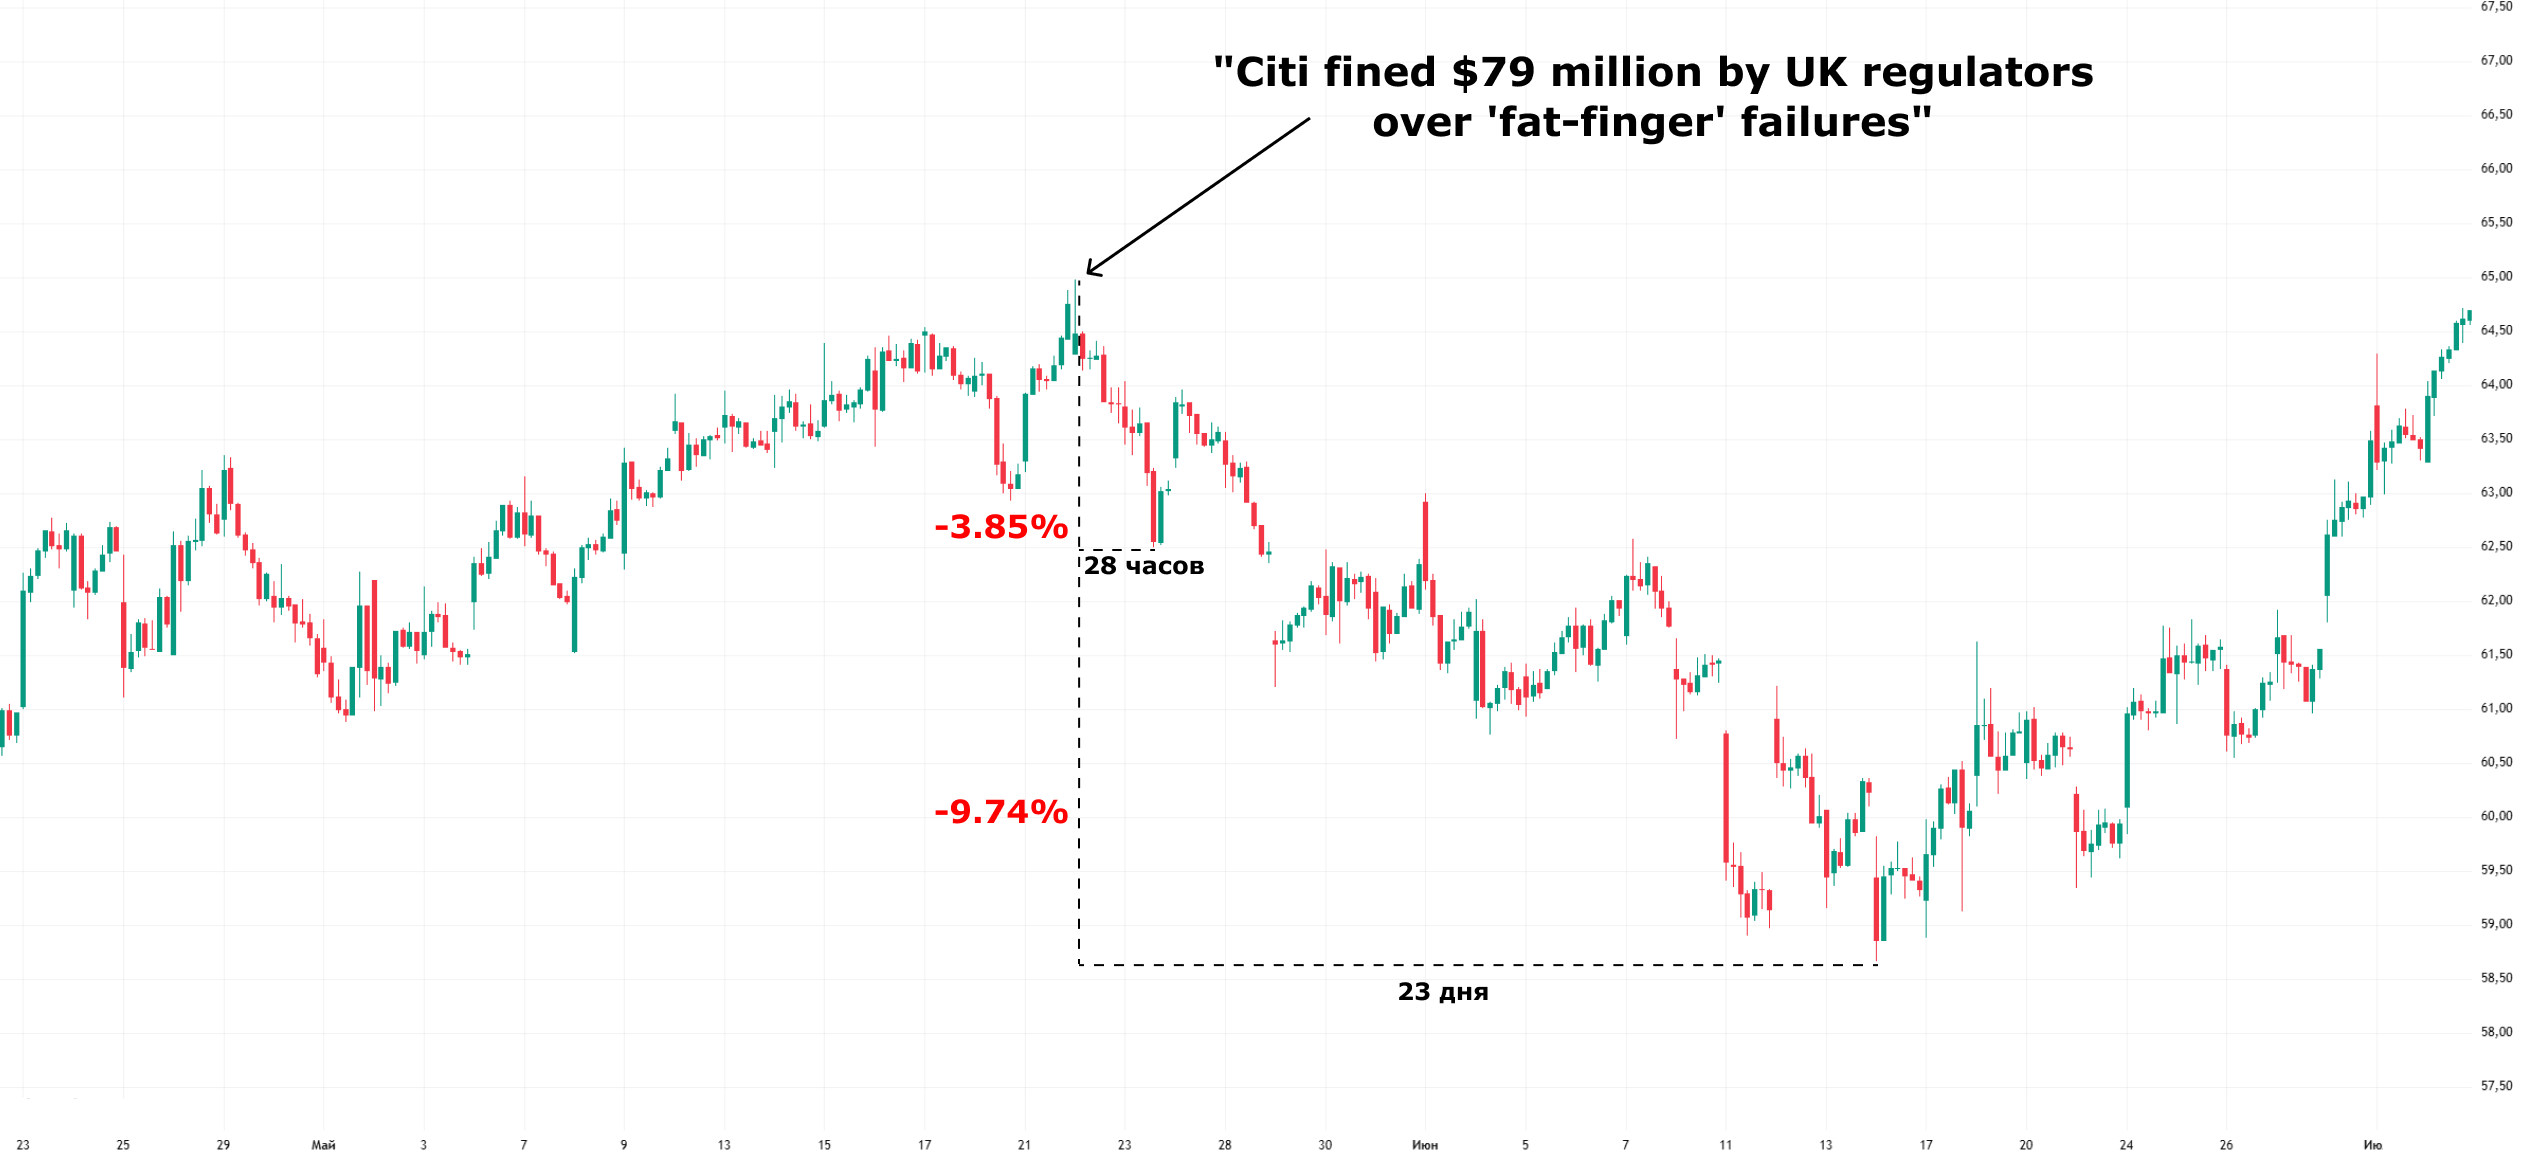
\includegraphics[width=1\linewidth]{img/citi_group.png}
    \caption{An example of the fall in the share price of one of the largest US banks, Citi Group
    (C.NYSE), due to allegations of insufficient control over trading operations, which caused
    a fall in European shares}
    \label{fig:citi_group}
\end{figure}

<<To be done later>>

\begin{figure}[H]
    \centering
    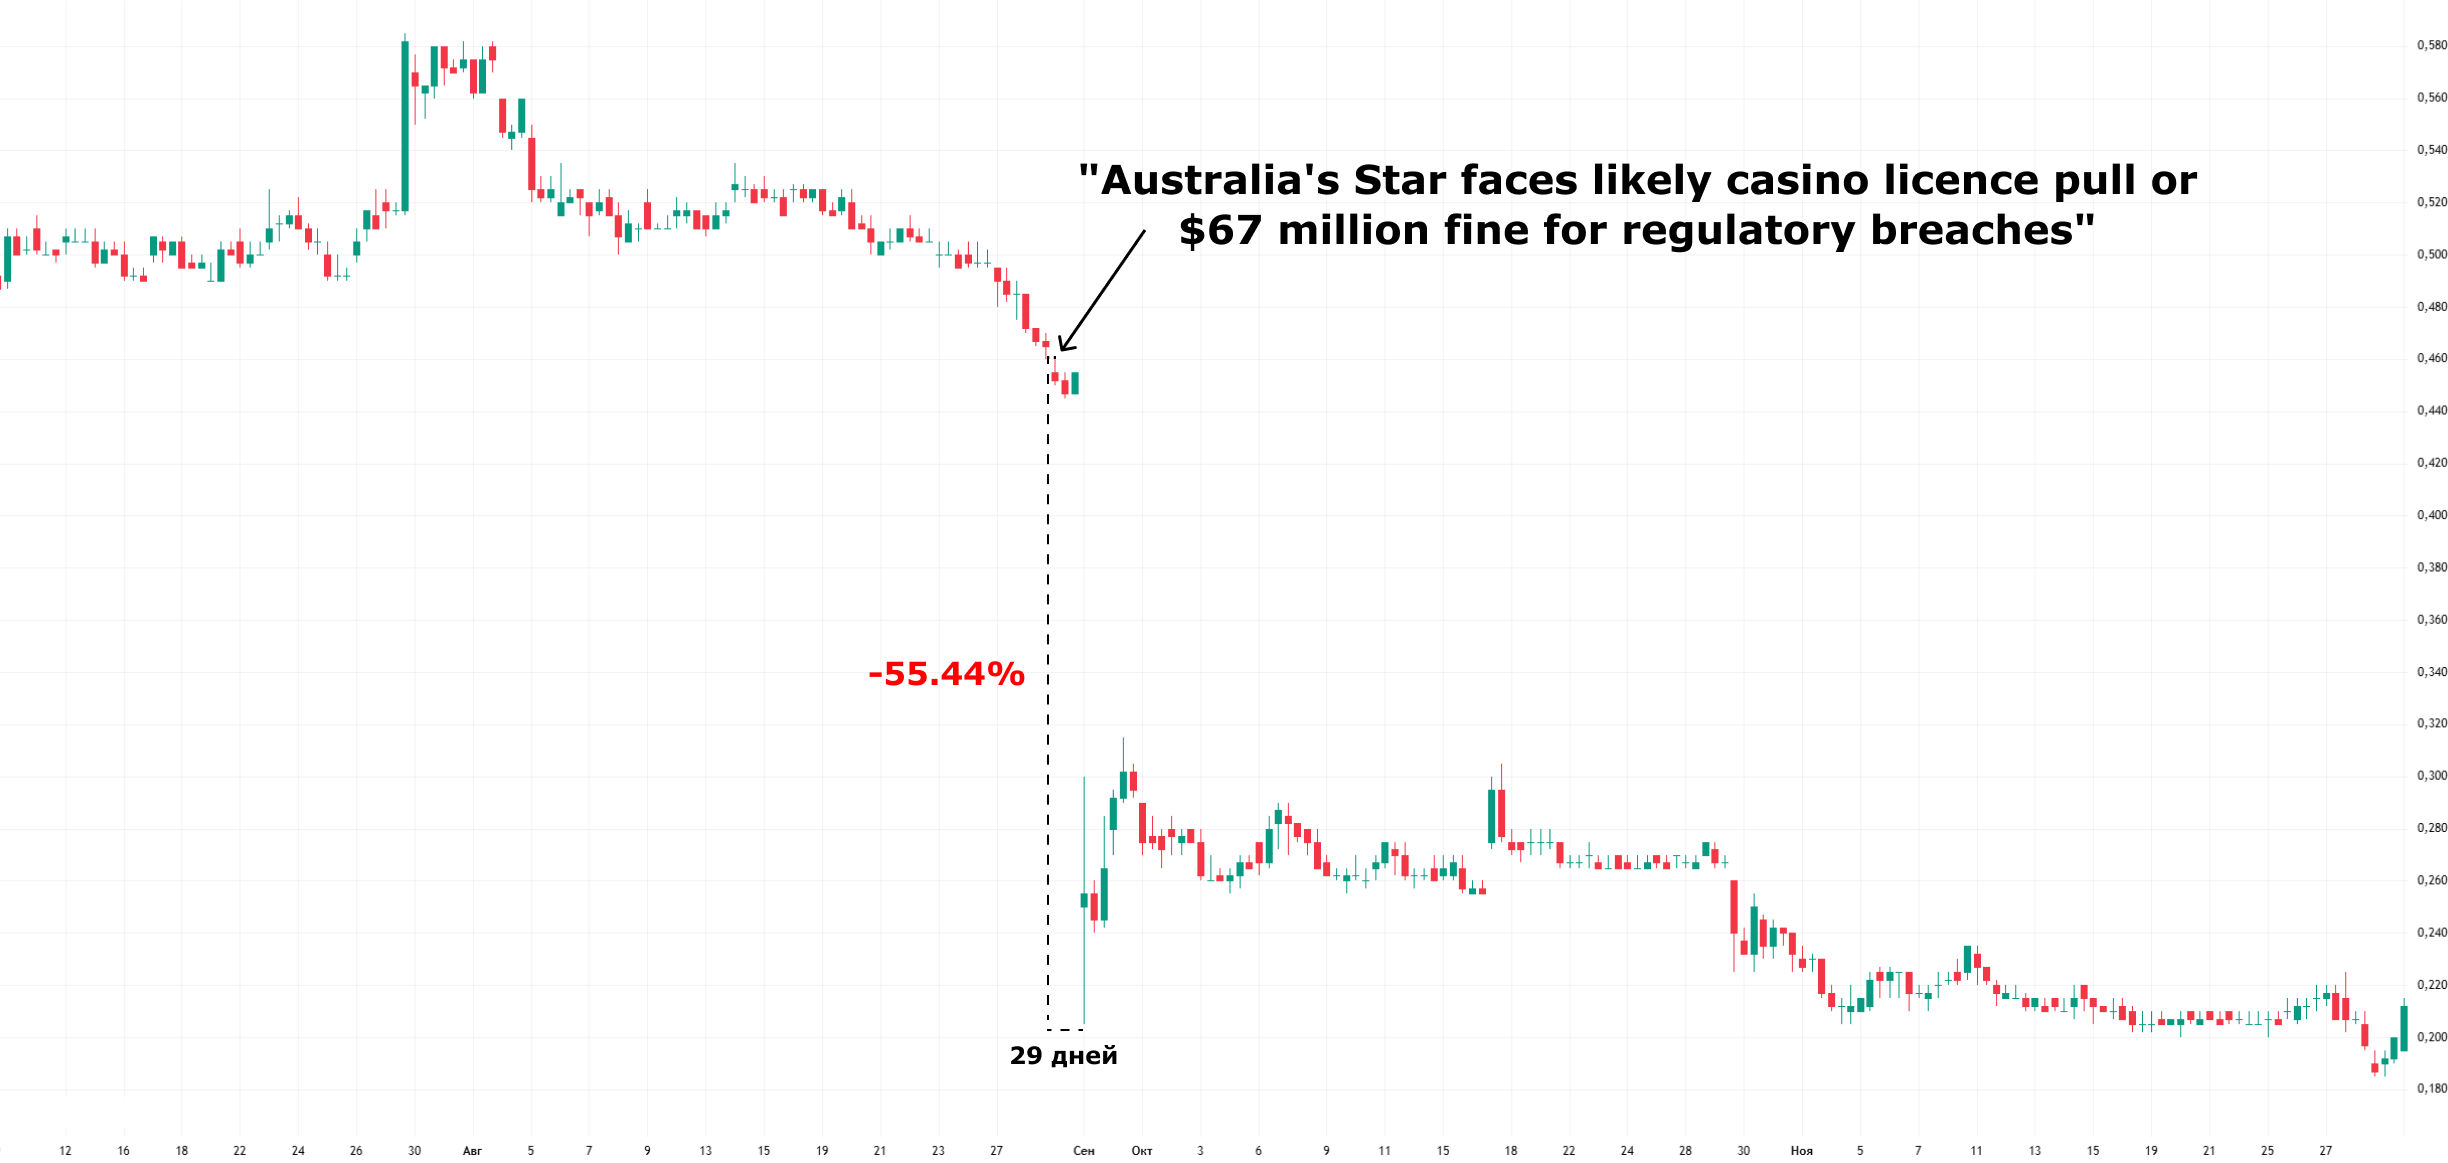
\includegraphics[width=1\linewidth]{img/star_entertainment.png}
    \caption{An example of Australian company The Star Entertainment Group LTD (SGR.ASX) shares
    collapsing and being temporarily halted from trading due to money laundering litigation.}
    \label{fig:star_entertainment}
\end{figure}